\documentclass[11pt,letterpaper]{article}
\usepackage[utf8]{inputenc}
\usepackage[T1]{fontenc}
\usepackage{mathptmx}
\usepackage[letterpaper,left=1.25in,right=1.25in,top=1.2in,bottom=1.2in,headheight=14pt]{geometry}
\usepackage{microtype}
\usepackage{amsmath,amssymb,amsthm,mathtools,bm}
\usepackage{graphicx,booktabs,array,multirow,float}
\usepackage{xcolor}
\usepackage{enumitem}
\usepackage[labelfont=bf,labelsep=colon,font=small,skip=4pt]{caption}
\usepackage{subcaption}
\usepackage{fancyhdr}
\usepackage{titlesec}
\usepackage{listings}
\usepackage{tikz}
\usetikzlibrary{arrows.meta,positioning,calc}
\usepackage[authoryear,round]{natbib}
\definecolor{linkcol}{HTML}{2B3A8F}
\usepackage[colorlinks=true,linkcolor=linkcol,citecolor=linkcol,urlcolor=linkcol]{hyperref}
\usepackage[capitalise,noabbrev]{cleveref}

\pagestyle{fancy}\fancyhf{}
\lhead{\small Technical report.}
\cfoot{\small\thepage}
\renewcommand{\headrulewidth}{0.5pt}
\setlength{\parskip}{4pt plus 1pt}\setlength{\parindent}{0pt}
\titleformat{\section}{\large\bfseries}{\thesection}{0.8em}{}
\titleformat{\subsection}{\normalsize\bfseries}{\thesubsection}{0.8em}{}
\titleformat{\subsubsection}{\normalsize\bfseries\itshape}{\thesubsubsection}{0.8em}{}
\titlespacing*{\section}{0pt}{16pt}{6pt}\titlespacing*{\subsection}{0pt}{12pt}{4pt}
\setlist{itemsep=1pt,topsep=3pt}
\setlength{\emergencystretch}{2em}

\theoremstyle{definition}
\newtheorem{definition}{Definition}
\theoremstyle{remark}
\newtheorem{remark}{Remark}

\lstset{basicstyle=\ttfamily\small,breaklines=true,frame=single,framerule=0.3pt,
  xleftmargin=4pt,xrightmargin=4pt,columns=fullflexible,keepspaces=true,showstringspaces=false}

% title block: \reporttitle{title}{subtitle}{authors}{affiliation line}
\newcommand{\reporttitle}[4]{%
\begin{center}
{\LARGE\bfseries #1\\[4pt]
\Large #2\par}
\vspace{1.4em}
{\bfseries\color{linkcol}\large #3}\\[0.4em]
{\small #4}\par
\vspace{1.2em}
\end{center}}
\newcommand{\abstractblock}[1]{%
\begin{center}\textbf{Abstract}\end{center}
\vspace{-0.4em}
\begin{quote}\small #1\end{quote}
\vspace{0.4em}}

\begin{document}
\reporttitle{How Fine Must the Mesh Be?}{Conjugate Heat Transfer in a Concentric Heat Exchanger,\\ Mesh Independence in 2D and 3D, and a Check Against Bench-Top Data}{Orsi Nagy \quad Juan Fernando Castaño}{Thermal Systems, New York University Abu Dhabi \quad $\cdot$ \quad \href{mailto:jfc9577@nyu.edu}{jfc9577@nyu.edu}}

\abstractblock{A finite-element heat-transfer result is only as good as its mesh, and the cost of a mesh grows quickly with its fineness. We built conjugate heat-transfer models of a concentric (tube-in-tube) water heat exchanger in COMSOL Multiphysics, first as an isothermal MEMS-scale block and then at laboratory scale (1\,m) in 3D and in a 2D axial section, and asked how fine the mesh actually has to be. In 3D we compared four predefined tetrahedral meshes over three inlet-temperature cases: the Fine and Extra fine meshes give the same profile, while the coarser ones over-predict the outlet temperature of the hot stream. In 2D we compared five structurally different meshes (free triangular, mapped rectangular, free quadrilateral). An extremely coarse unstructured triangular mesh of 47\,210 elements matches the 86\,520-element reference, whereas a mapped mesh with the most elements, 108\,000, produced a physically implausible, nearly flat hot-channel profile. The selected mesh was compared with measurements from a bench-top shell-and-tube unit; the agreement is qualitative and limited to the hot-channel outlet. A solver discrepancy on one 3D mesh, which we could not explain, is reported and not hidden.}

\section{Introduction}
Mesh refinement is the most routine check in computational heat transfer and the one most often skipped, because every refinement costs solver time and the answer usually looks plausible either way. In this project the answer did not look plausible for every mesh, and that is why the check was worth running.

The system is a concentric tube exchanger, an inner tube and an outer annulus carrying two water streams, with heat moving from the hot to the cold stream through a thin copper wall. It is a standard teaching geometry with a well-understood answer, so it is a good place to ask two questions about the model and not about the physics.

\textbf{Question 1: how fine does the mesh need to be?} We compare mesh families of different type and density, in 3D and in 2D, and look for the point beyond which the temperature profile stops changing. The question has a cost side: in 2D we also ask whether a cheaper mesh gives the same answer as the reference.

\textbf{Question 2: does the selected model agree with a real exchanger?} A mesh-independent solution can still be wrong. We compare the model with measured inlet and outlet temperatures from a bench-top shell-and-tube unit.

\textbf{What we find.} In 3D, Fine and Extra fine coincide in all three cases, and Extra coarse and Normal over-predict the hot outlet temperature. In 2D, an extremely coarse triangular mesh agrees with the reference at 55\% of the elements, and element count is a poor predictor of quality: the largest mesh gave the worst profile. The model is consistent with the bench-top outlet temperature, but we can say this only qualitatively.

\textbf{Contributions.} We do not propose a new method. Our contributions are:
\begin{enumerate}
\item A mesh-independence study with nine meshes (four in 3D, five in 2D) over three inlet-temperature cases, reported with element counts (\cref{sec:results}).
\item A documented counter-example in which the mesh with the most elements gives the least credible profile.
\item A solver discrepancy on one 3D mesh, described with enough detail for someone else to look for it (\cref{sec:anomaly}).
\item A qualitative verification against bench-top data, with its limits stated (\cref{sec:verify}).
\end{enumerate}

\textbf{Organisation.} \Cref{sec:background} gives background, \cref{sec:models} the models and \cref{sec:protocol} the study protocol. \Cref{sec:results} presents the results and \cref{sec:discussion} states what they establish.

\section{Background}\label{sec:background}
\textbf{Heat exchangers.} In a concentric exchanger the heat duty is set by the stream temperatures, the flow rates and the overall resistance made up of two convective films and the wall conduction \citep{incropera2007,shah2003,kays1984}. In a conjugate model the solid wall and both fluids are solved together, so the film resistances emerge from the flow and temperature fields and are not supplied by correlations.

\textbf{Discretisation error.} A finite-element solution carries an error that falls as the mesh is refined, and the standard practice is to show that the quantity of interest no longer changes appreciably between successive meshes \citep{roache1998,celik2008}. Formal procedures use a systematic refinement ratio and an error estimate; our meshes are predefined or hand-built and are not related by a constant ratio, so we use the simpler comparison of profiles.

\textbf{Mesh type.} Structured (mapped) meshes are often preferred for their regularity, but regularity does not guarantee a good solution: what matters is how well the elements resolve the gradients near the wall. The 2D result below is an example.

\section{Models}\label{sec:models}
\subsection{Part A: isothermal MEMS-scale exchanger}
The first model is a small rectangular block containing a hot and a cold circular channel. It served to learn the solver and to see how boundary temperatures shape the field. Four hot/cold temperature pairs were run, 330/300, 363/300, 330/270 and 363/270\,K, and eight mesh densities from extremely coarse to extremely fine were compared on the hot-channel centreline temperature over a 400\,\textmu m arc length (\cref{fig:mems}).
\begin{figure}[t]\centering
\begin{subfigure}{0.31\linewidth}\centering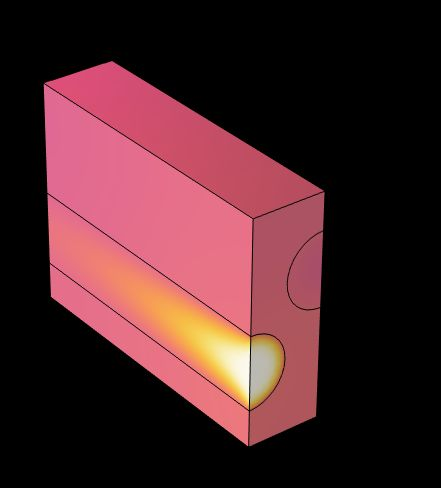
\includegraphics[width=\linewidth]{figures/mems_iso.png}\caption{Temperature field.}\end{subfigure}\hfill
\begin{subfigure}{0.31\linewidth}\centering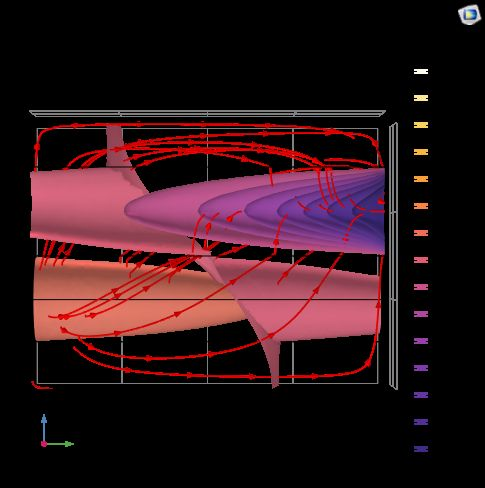
\includegraphics[width=\linewidth]{figures/mems_stream_a.png}\caption{Streamlines and isosurfaces.}\end{subfigure}\hfill
\begin{subfigure}{0.31\linewidth}\centering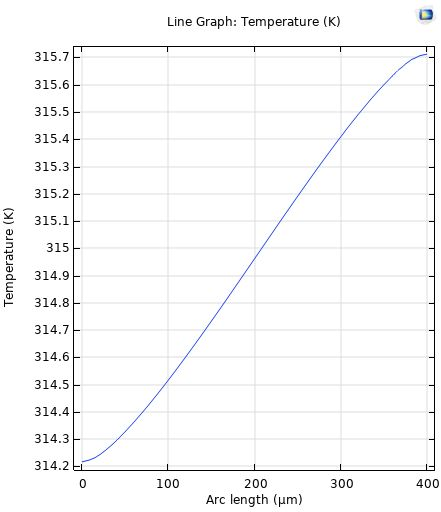
\includegraphics[width=\linewidth]{figures/mems_line.png}\caption{Centreline temperature.}\end{subfigure}
\caption{MEMS-scale model with a 330\,K hot channel and a 300\,K cold channel.}\label{fig:mems}
\end{figure}

\subsection{Part B: concentric exchanger at laboratory scale}
The exchanger is 1\,m long. The hot channel has a radius of 1.25\,cm and the cold annulus an outer radius of 2.5\,cm, separated by a copper wall of about 1\,mm, which we assume is thin enough not to change the channel radii. Both streams have a uniform (plug) velocity profile. The whole outer surface is insulated ($Q=0$); the hot channel inlet is held at $T_{\mathrm{hot}}$ and the cold channel inlet at $T_{\mathrm{cold}}$. Temperature is sampled along a line through the middle of the geometry. The 3D model and the 2D axial section are shown in \cref{fig:geom}.
\begin{figure}[t]\centering
\begin{subfigure}{0.34\linewidth}\centering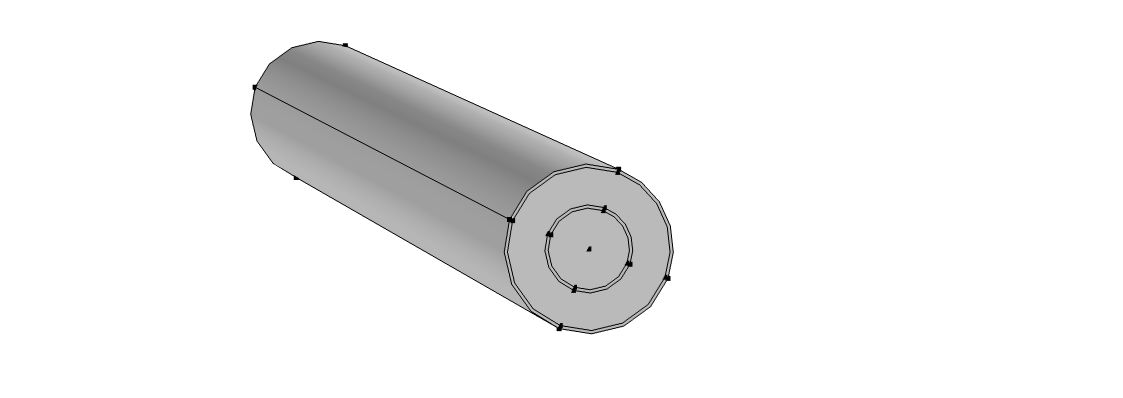
\includegraphics[width=\linewidth]{figures/geom3d.png}\caption{3D geometry.}\end{subfigure}\hfill
\begin{subfigure}{0.60\linewidth}\centering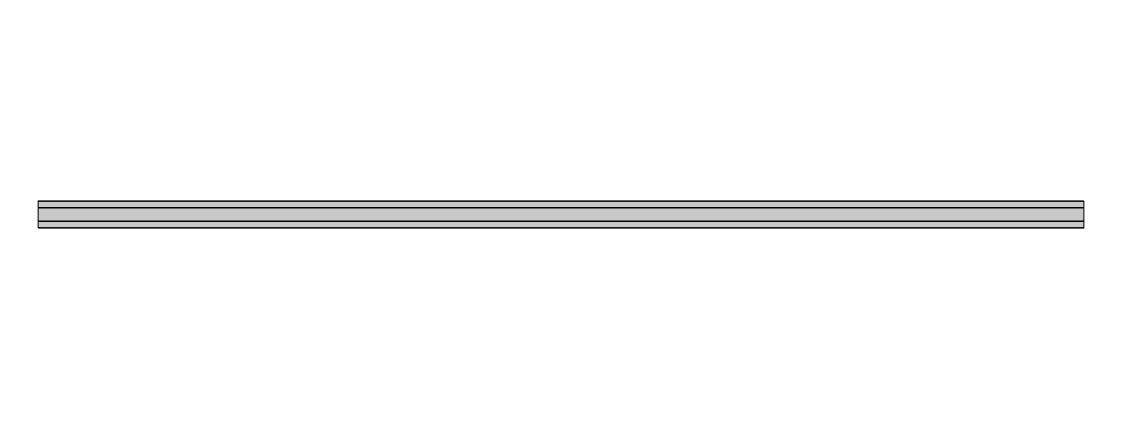
\includegraphics[width=\linewidth]{figures/geom2d.png}\caption{2D axial section, centred at the origin.}\end{subfigure}
\caption{Geometry used in COMSOL \citep{comsol}.}\label{fig:geom}
\end{figure}

\subsection{Meshes}
In 3D, four predefined free-tetrahedral meshes were generated: Extra coarse, Normal, Fine and Extra fine. In 2D we built five meshes of different structure, listed in \cref{tab:mesh2d} with the resulting case-1 hot-channel exit temperature.
\begin{table}[t]\centering\small
\begin{tabular}{@{}llrrr@{}}\toprule
Mesh & Type & Domain el. & Boundary el. & Exit $T$ (K)\\\midrule
1 & Free triangular, $h_{\max}=2$\,mm & 86\,520 & 12\,016 & 317.7\\
2 & Free triangular, extremely coarse & 47\,210 & 10\,463 & 312.4\\
3 & Mapped rectangular, $h_{\max}=0.5$\,mm & 108\,000 & 18\,108 & $\approx$\,320\\
4 & Free quadrilateral, extra fine & 41\,416 & 12\,016 & 318.0\\
5 & Free quadrilateral, 5\,mm--0.12\,m & 33\,593 & 11\,740 & 315.4\\\bottomrule
\end{tabular}
\caption{The five 2D meshes and the case-1 hot-channel exit temperature read from the COMSOL line graphs. Mesh 3 shows no temperature drop along the channel.}\label{tab:mesh2d}
\end{table}

\section{Study Protocol}\label{sec:protocol}
Each mesh was solved for three hot-inlet cases. The case temperatures, read from the plot axes, are 320, 315 and 310\,K with a cold inlet of 300\,K. Profiles are compared along the centreline. For verification we used a bench-top shell-and-tube service unit (\cref{fig:rig}) that recorded a hot-channel inlet of 313.5\,K and an outlet of 311.5\,K. The 2D meshes were started from the measured hot inlet temperature and compared at the outlet.
\begin{figure}[t]\centering
\begin{subfigure}{0.42\linewidth}\centering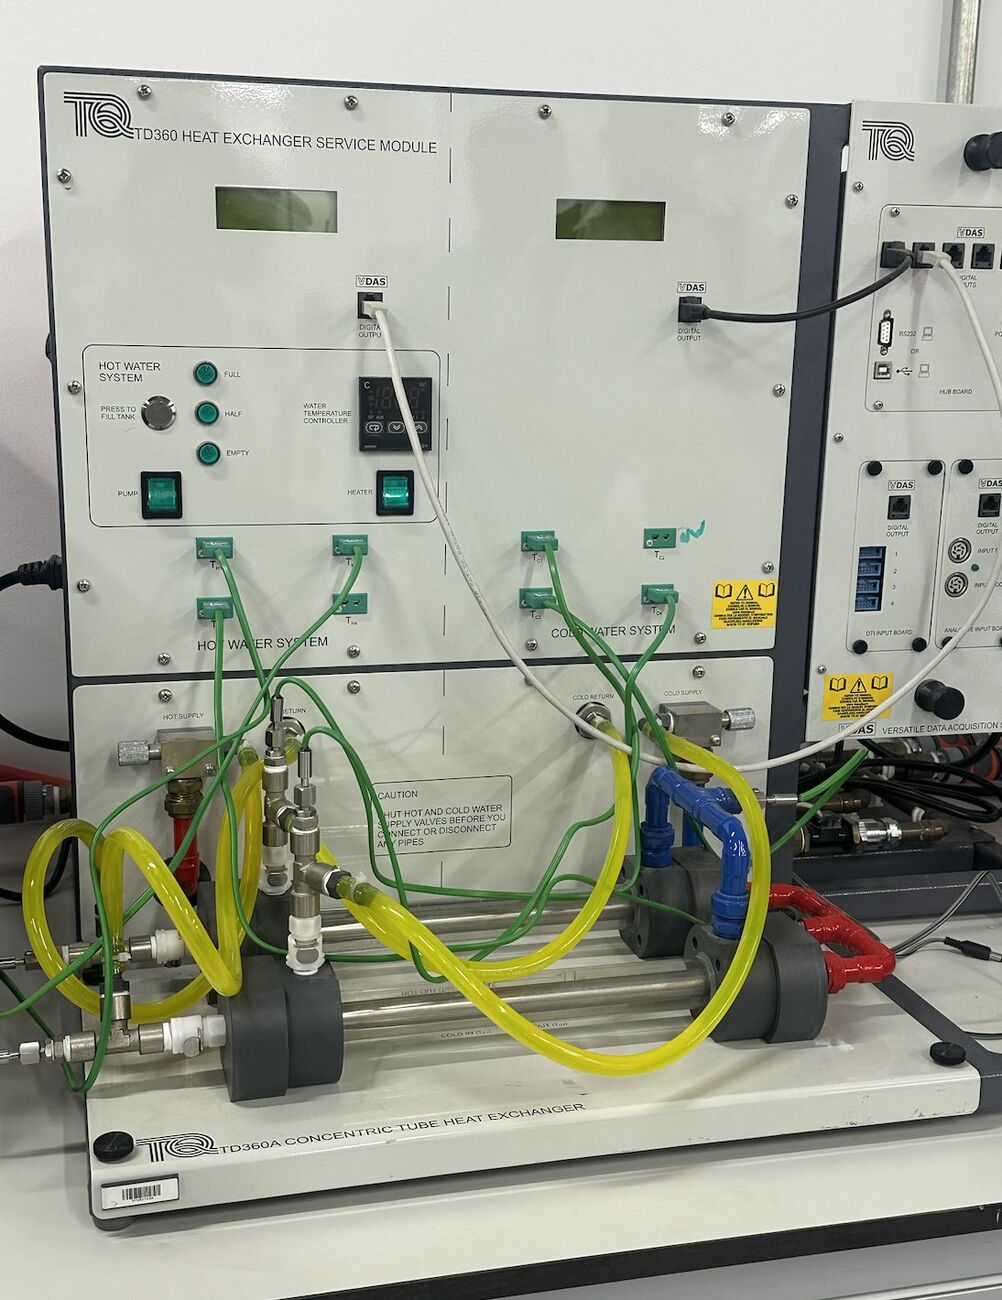
\includegraphics[width=\linewidth]{figures/rig_overview.jpg}\caption{Bench-top service unit.}\end{subfigure}\hfill
\begin{subfigure}{0.42\linewidth}\centering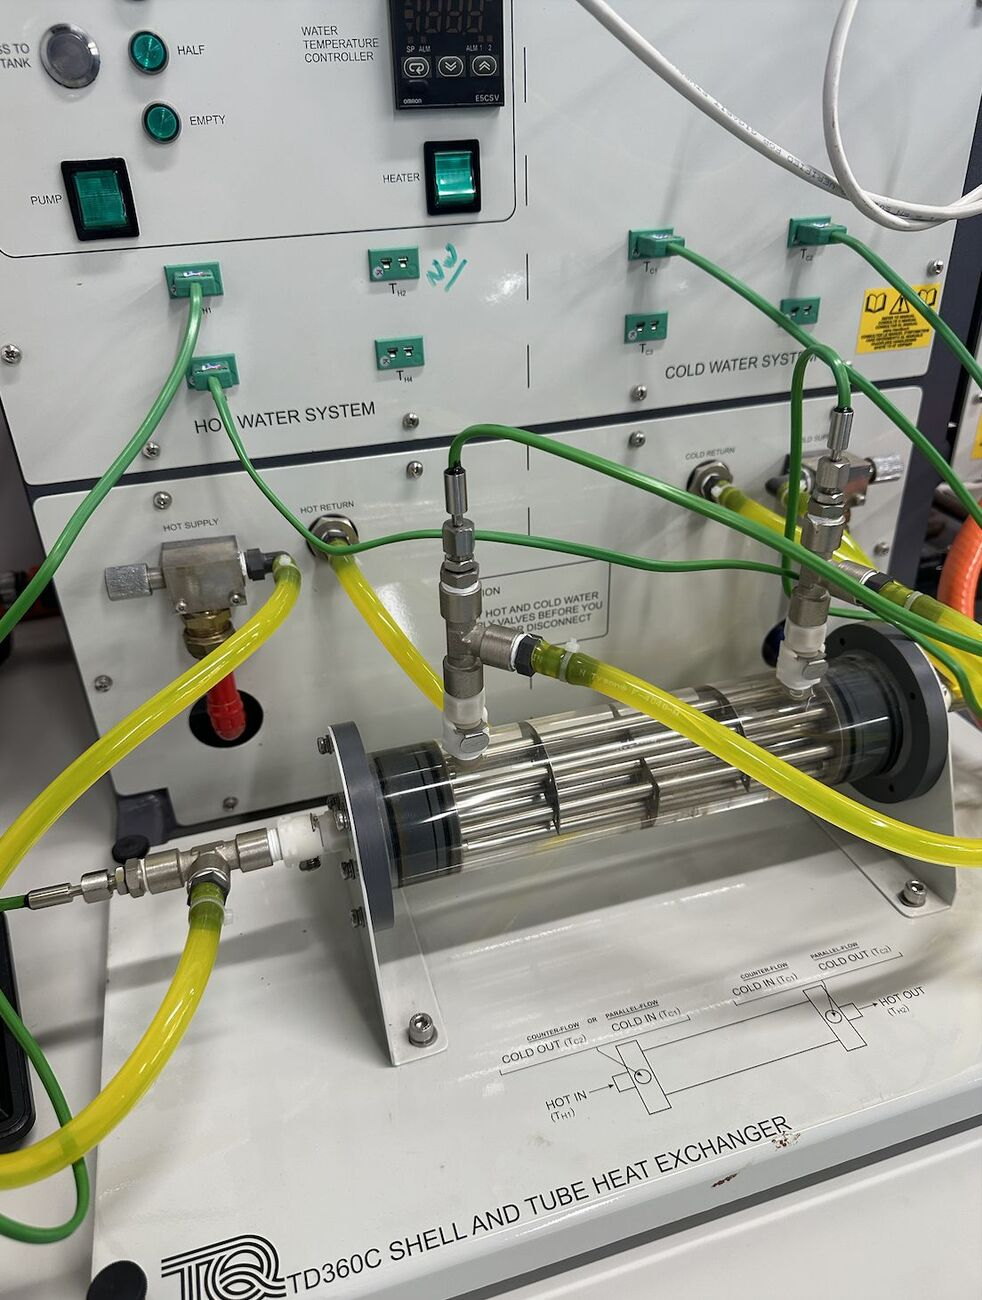
\includegraphics[width=\linewidth]{figures/rig_closeup.jpg}\caption{Shell-and-tube section with thermocouple ports.}\end{subfigure}
\caption{Apparatus that supplied the verification data.}\label{fig:rig}
\end{figure}

\section{Results}\label{sec:results}
\subsection{3D mesh independence}
\Cref{fig:ind3d} shows the centreline temperature for the four 3D meshes in the three cases. Fine and Extra fine coincide in every case. Extra coarse and Normal sit well above them: the coarse meshes under-resolve the thermal boundary layer at the wall, under-predict the heat transferred to the cold stream, and therefore over-predict the temperature at which the hot stream leaves. The individual meshes and their profiles are in \cref{app:meshes}.
\begin{figure}[t]\centering
\begin{subfigure}{0.48\linewidth}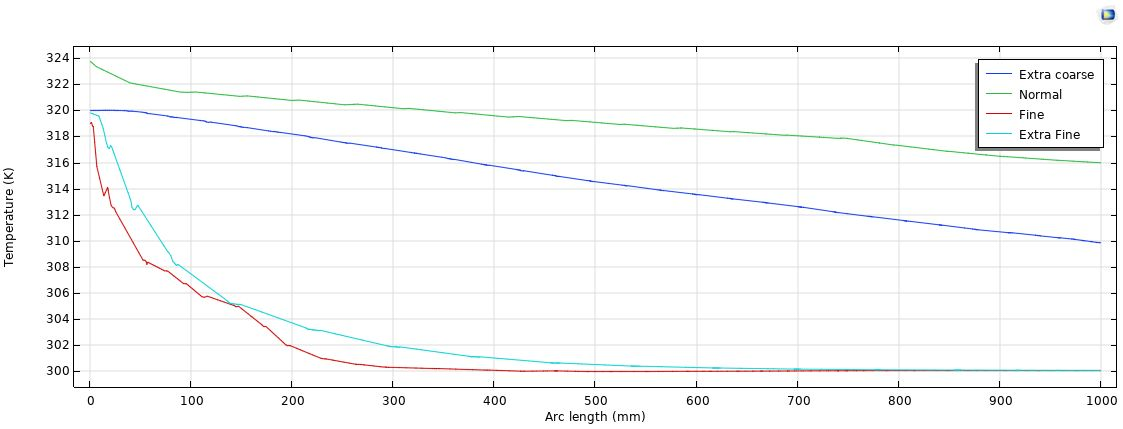
\includegraphics[width=\linewidth]{figures/ind3d_c1.png}\caption{Case 1.}\end{subfigure}\hfill
\begin{subfigure}{0.48\linewidth}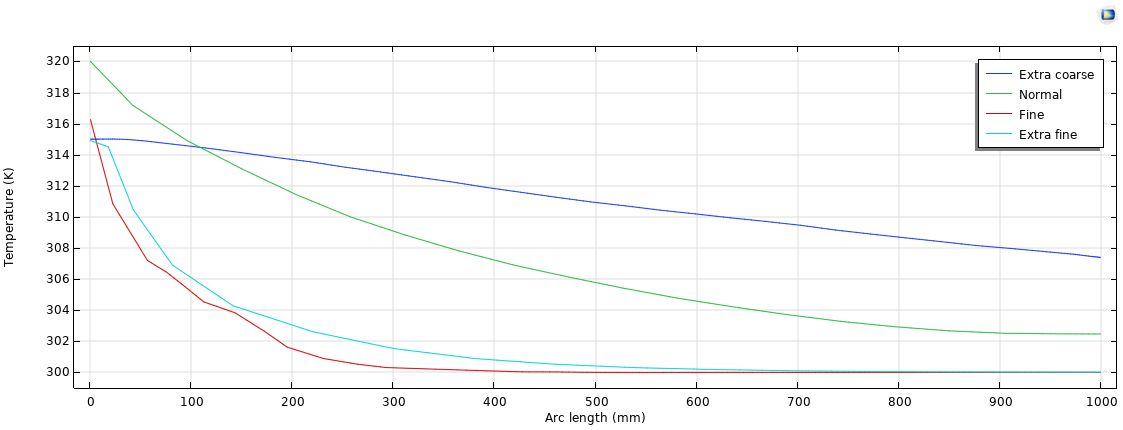
\includegraphics[width=\linewidth]{figures/ind3d_c2.png}\caption{Case 2.}\end{subfigure}\\[4pt]
\begin{subfigure}{0.48\linewidth}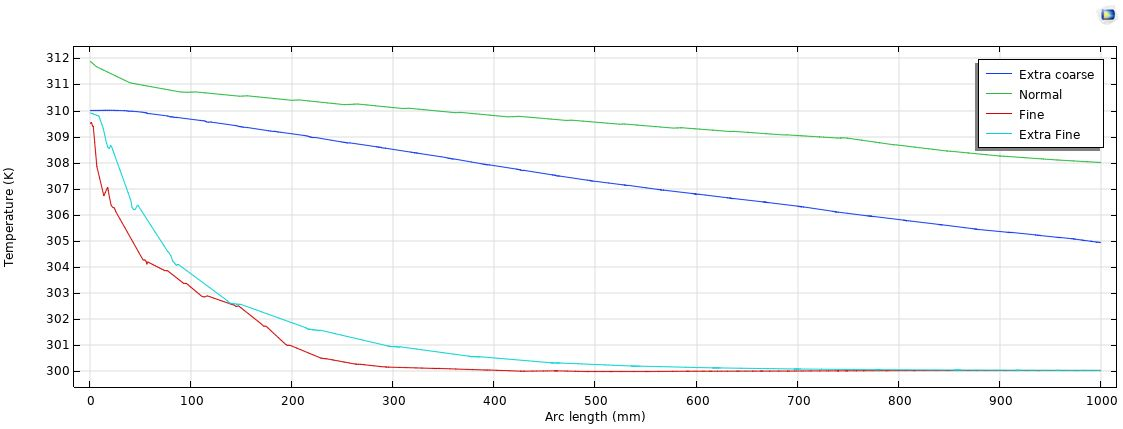
\includegraphics[width=\linewidth]{figures/ind3d_c3.png}\caption{Case 3.}\end{subfigure}
\caption{3D mesh independence. The Fine and Extra fine curves coincide in all three cases.}\label{fig:ind3d}
\end{figure}

\subsection{An unresolved solver discrepancy}\label{sec:anomaly}
Temperature plots differed depending on whether meshes were computed one at a time or several together, both on a Line Segment and on a Cut Line. The effect mainly hit the Normal mesh and made the hot-channel inlet temperature higher than the parameter that had been set. We could not identify the cause and consider the error too large to blame on endpoint round-off. We therefore used a mesh that was not affected. The cause should be investigated before the Normal-mesh result is used for anything.

\subsection{2D mesh independence}
\Cref{fig:ind2d} compares Meshes 1, 2, 4 and 5 in the three cases. Meshes 1 and 2 agree with each other in every case, although Mesh 2 has 55\% of the elements, so Mesh 2 was used throughout. The mapped rectangular mesh (Mesh 3) is not in the comparison: it has the most elements, 108\,000, and gave an almost flat hot-channel profile with no temperature drop, which is not physical for this exchanger. Element count is therefore not a measure of quality. Mesh details for all five are in \cref{app:meshes}.
\begin{figure}[t]\centering
\begin{subfigure}{0.48\linewidth}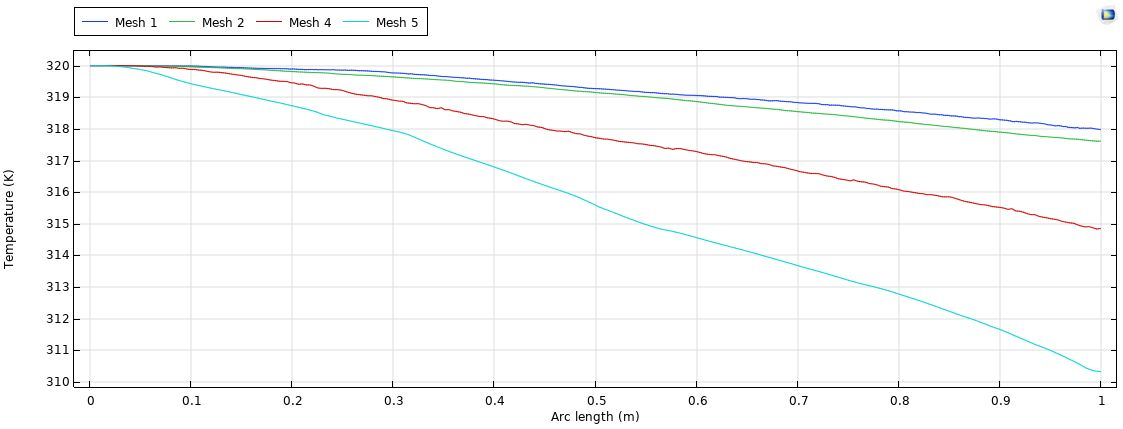
\includegraphics[width=\linewidth]{figures/ind2d_c1.png}\caption{Case 1.}\end{subfigure}\hfill
\begin{subfigure}{0.48\linewidth}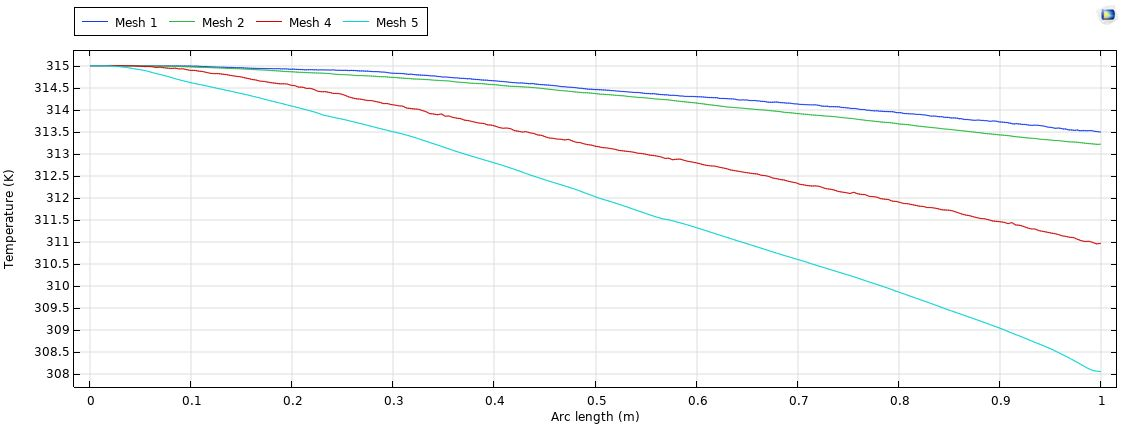
\includegraphics[width=\linewidth]{figures/ind2d_c2.png}\caption{Case 2.}\end{subfigure}\\[4pt]
\begin{subfigure}{0.48\linewidth}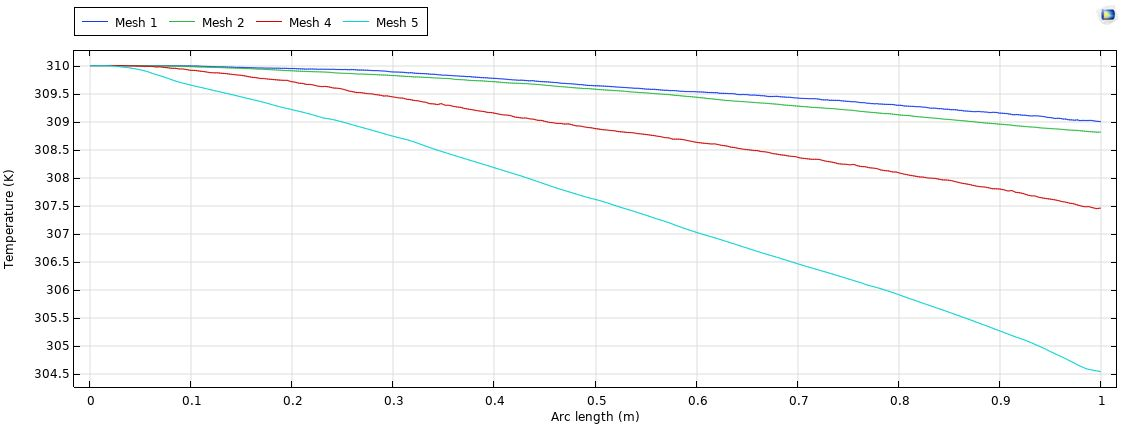
\includegraphics[width=\linewidth]{figures/ind2d_c3.png}\caption{Case 3.}\end{subfigure}
\caption{2D mesh independence for Meshes 1, 2, 4 and 5.}\label{fig:ind2d}
\end{figure}

\subsection{Comparison with the bench-top unit}\label{sec:verify}
\Cref{fig:verify} shows the 2D profiles started from the measured hot inlet temperature of 313.5\,K. Of the candidate meshes, Mesh 2 matched the measured outlet of 311.5\,K most closely. The comparison is at the hot-channel outlet only and the source material gives no residual, so we describe the agreement as qualitative.
\begin{figure}[t]\centering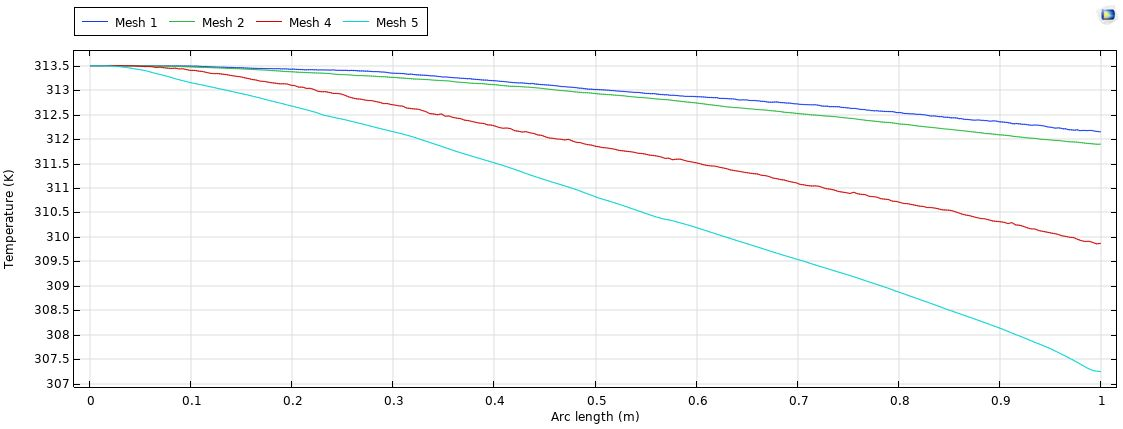
\includegraphics[width=0.72\linewidth]{figures/verify2d.png}
\caption{Verification run: model profiles for Meshes 1, 2, 4 and 5 started from the measured hot-inlet temperature.}\label{fig:verify}
\end{figure}

\section{Discussion}\label{sec:discussion}
\textbf{Mesh choice matters at the level of kelvin.} Across the meshes tried, the predicted hot-outlet temperature differs by several kelvin, which is large against the 2\,K drop measured on the bench. A mesh-independence check is therefore part of the result, not a preliminary to it.

\textbf{Practical consequences.} In 3D, the Fine mesh is sufficient. In 2D, an extremely coarse unstructured triangular mesh is already converged for this geometry and halves the cost. Do not rely on element count as a proxy for quality, and look at the profile before trusting the number.

\textbf{What this study does not establish.} The experimental comparison covers the hot-channel outlet only and is qualitative. The case temperatures and the 2D exit temperatures were read from COMSOL plots, not from exported tables, so they carry reading error. The 3D Normal-mesh discrepancy is unexplained. The meshes are not related by a constant refinement ratio, so we give no formal discretisation-error estimate. We assumed plug flow in both channels, a thin copper wall and an insulated outer surface; none of these was tested. We did not run counter-current flow or an effectiveness--NTU cross-check.

\textbf{Next steps.} Resolve the Normal-mesh discrepancy, replace the plug-flow assumption with a fully developed laminar profile, compare the cold-side outlet and the overall heat duty with the bench data, and add counter-current runs with an effectiveness--NTU check.

\textbf{Conclusion.} For a concentric exchanger, mesh quality and not mesh size decides the answer. The Fine 3D mesh and an extremely coarse unstructured 2D mesh give converged centreline profiles, a 108\,000-element mapped mesh does not, and the converged model is consistent with the one outlet temperature we measured.

\section*{Code and data availability}
The report source, the figures exported from COMSOL and the notes on how each case was set up are in the repository accompanying it. The COMSOL model files are not included.

\bibliographystyle{plainnat}
\bibliography{references}

\appendix
\section{Mesh Details}\label{app:meshes}
\begin{figure}[H]\centering
\setlength{\tabcolsep}{2pt}
\begin{tabular}{cc}
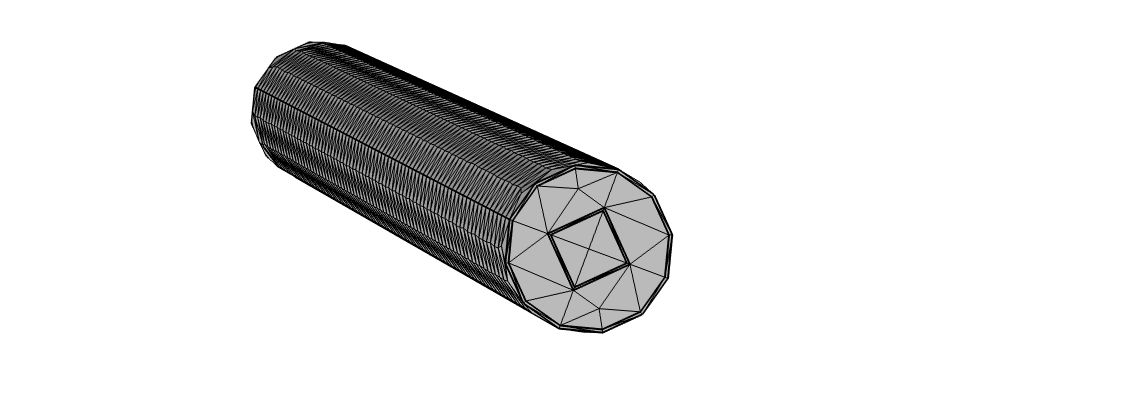
\includegraphics[width=0.14\linewidth]{figures/m3d_1_mesh.png}\ \ 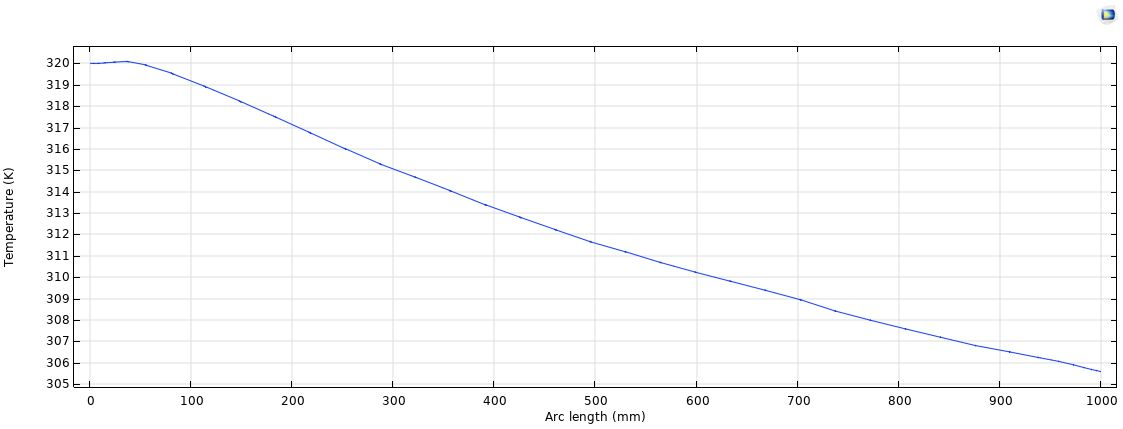
\includegraphics[width=0.40\linewidth]{figures/m3d_1_prof.png} & 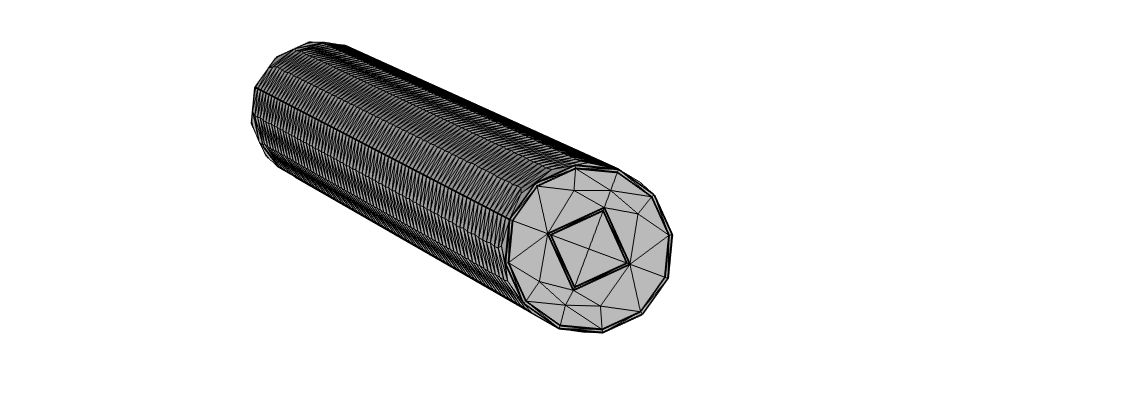
\includegraphics[width=0.14\linewidth]{figures/m3d_2_mesh.png}\ \ 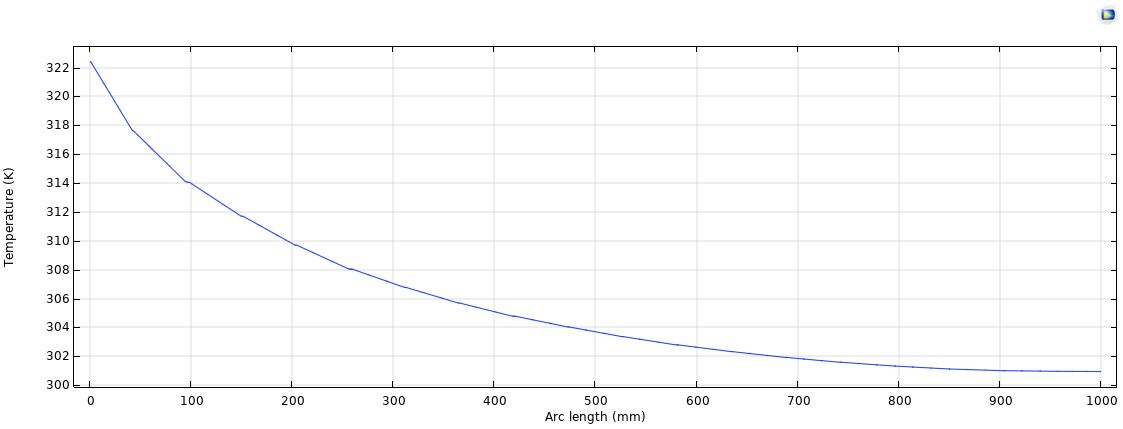
\includegraphics[width=0.40\linewidth]{figures/m3d_2_prof.png}\\
{\small (a) Mesh 1, Extra coarse} & {\small (b) Mesh 2, Normal}\\[4pt]
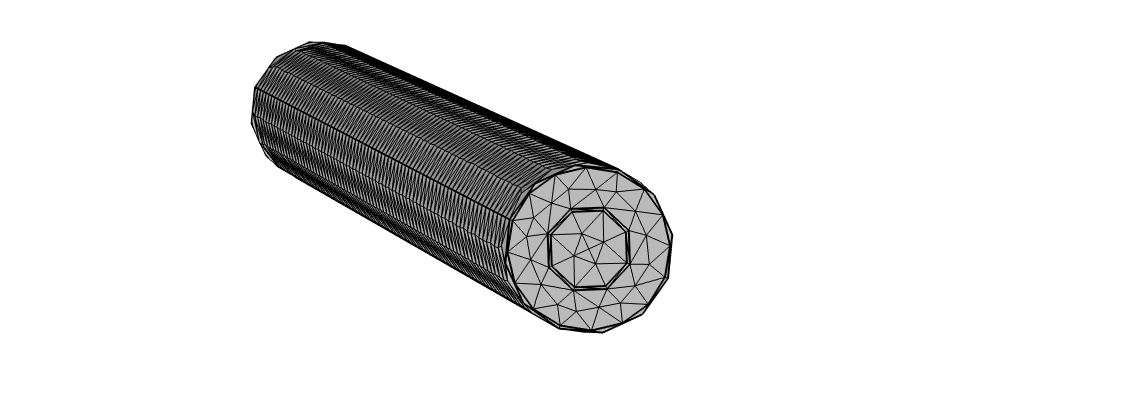
\includegraphics[width=0.14\linewidth]{figures/m3d_3_mesh.png}\ \ 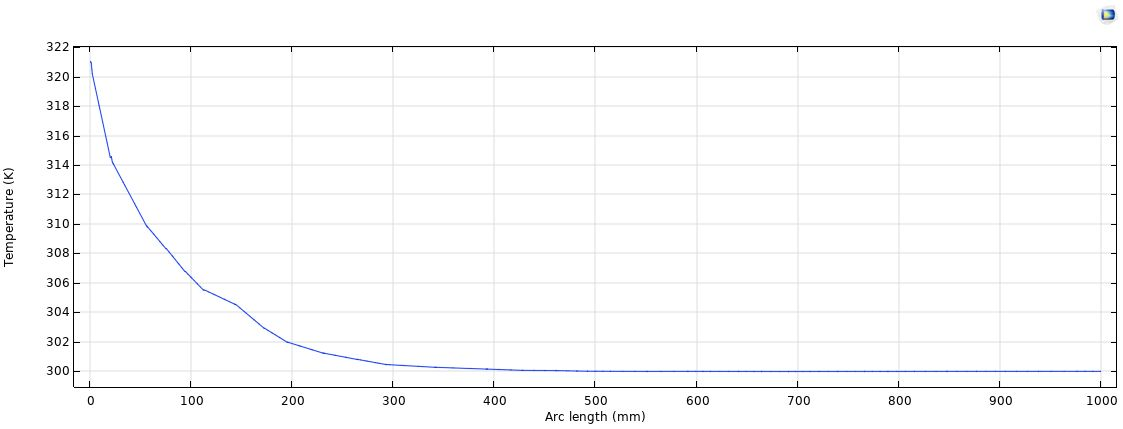
\includegraphics[width=0.40\linewidth]{figures/m3d_3_prof.png} & 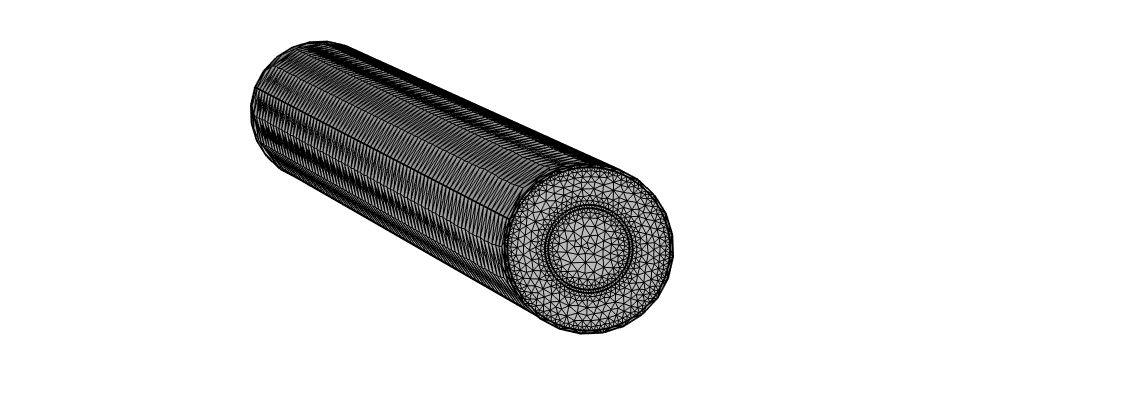
\includegraphics[width=0.14\linewidth]{figures/m3d_4_mesh.png}\ \ 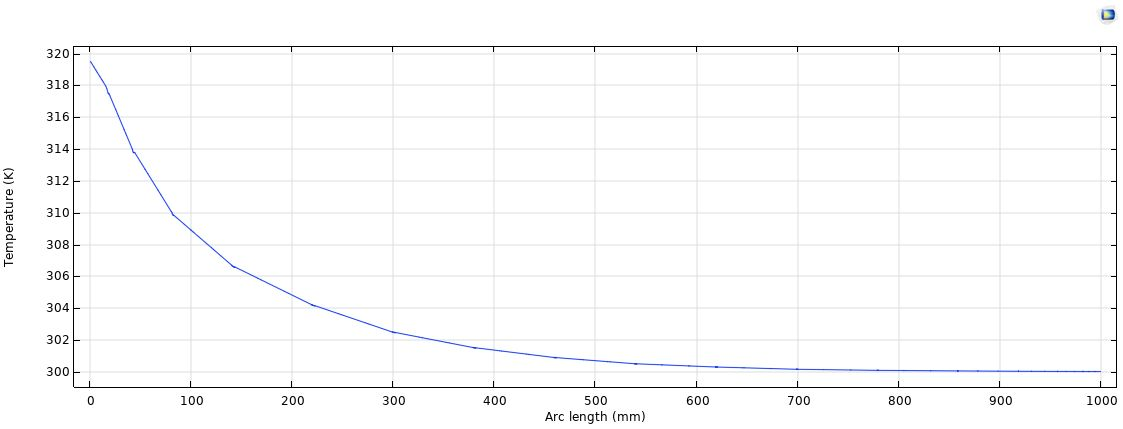
\includegraphics[width=0.40\linewidth]{figures/m3d_4_prof.png}\\
{\small (c) Mesh 3, Fine} & {\small (d) Mesh 4, Extra fine}
\end{tabular}
\caption{3D meshes and the case-1 centreline temperature profiles.}
\end{figure}
\begin{figure}[H]\centering
\setlength{\tabcolsep}{2pt}
\begin{tabular}{cc}
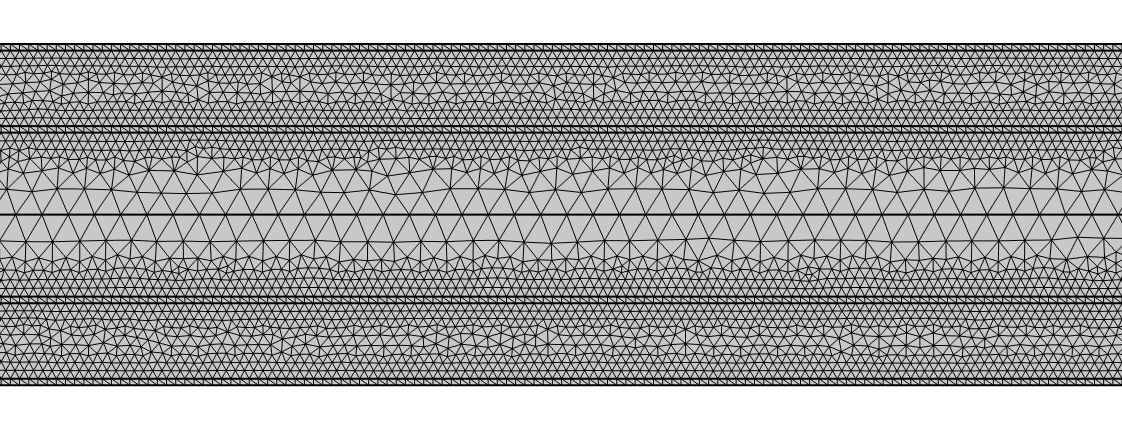
\includegraphics[width=0.47\linewidth]{figures/m2d_1_mesh.jpg} & 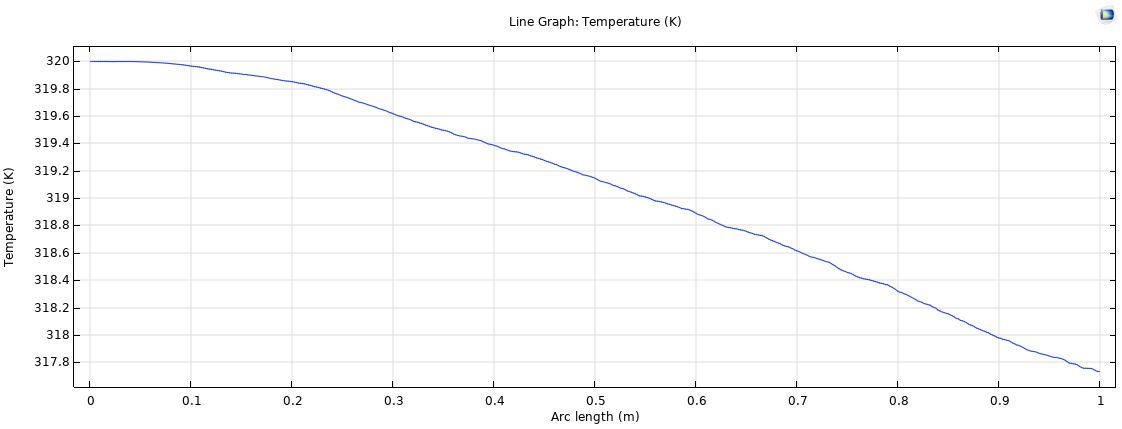
\includegraphics[width=0.47\linewidth]{figures/m2d_1_prof.png}\\
\multicolumn{2}{c}{\small Mesh 1: free triangular}\\[3pt]
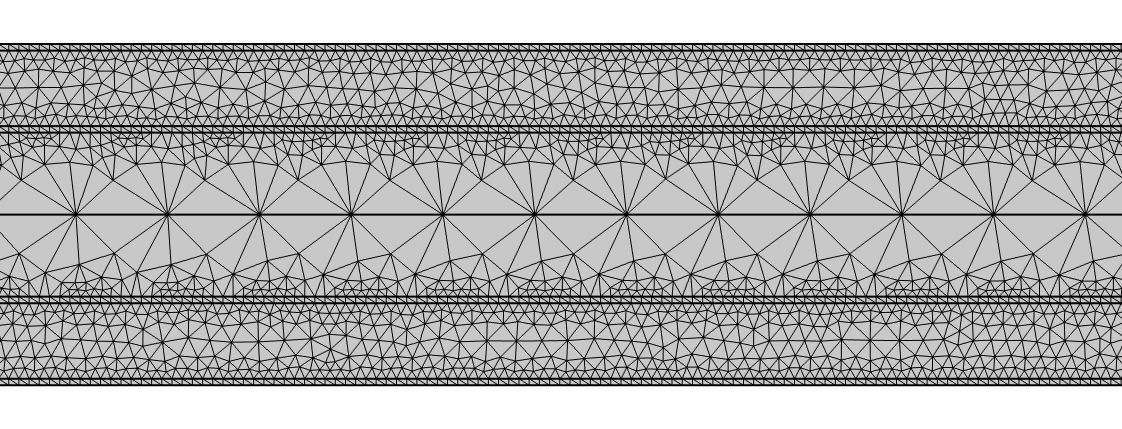
\includegraphics[width=0.47\linewidth]{figures/m2d_2_mesh.jpg} & 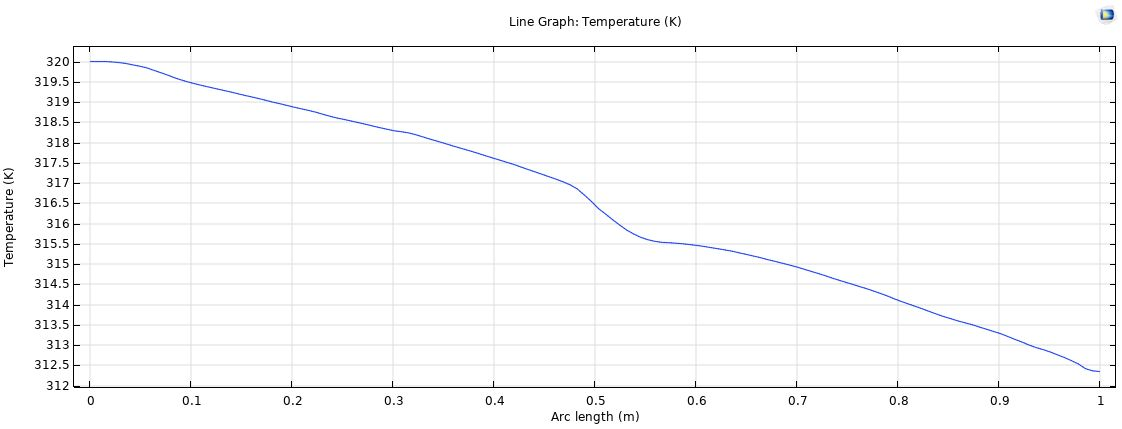
\includegraphics[width=0.47\linewidth]{figures/m2d_2_prof.png}\\
\multicolumn{2}{c}{\small Mesh 2: extremely coarse}\\[3pt]
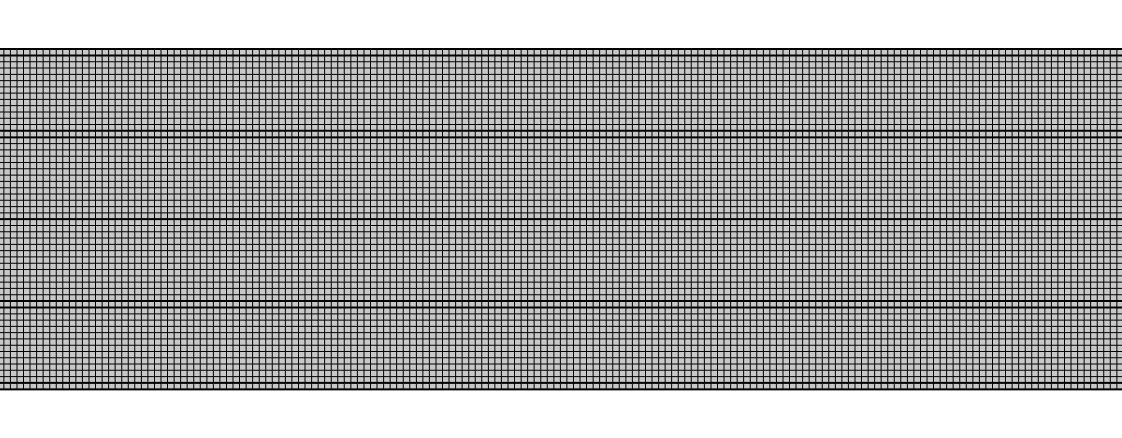
\includegraphics[width=0.47\linewidth]{figures/m2d_3_mesh.png} & 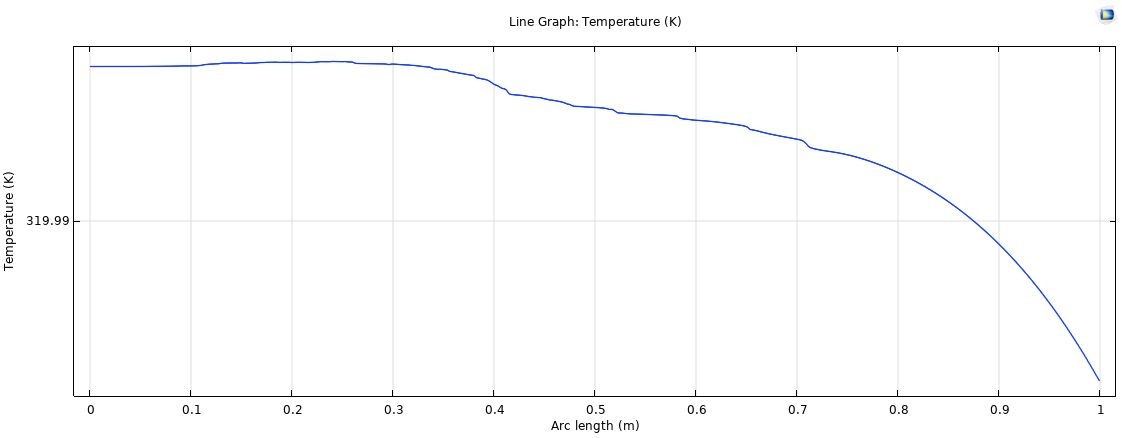
\includegraphics[width=0.47\linewidth]{figures/m2d_3_prof.png}\\
\multicolumn{2}{c}{\small Mesh 3: mapped rectangular}
\end{tabular}
\caption{2D Meshes 1 to 3: mesh detail on the left, centreline temperature on the right.}
\end{figure}
\begin{figure}[H]\centering
\setlength{\tabcolsep}{2pt}
\begin{tabular}{cc}
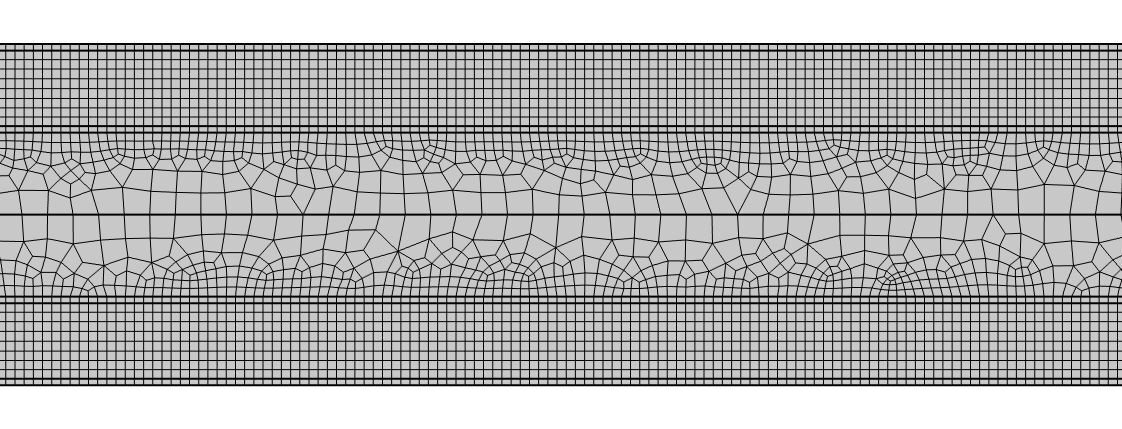
\includegraphics[width=0.47\linewidth]{figures/m2d_4_mesh.jpg} & 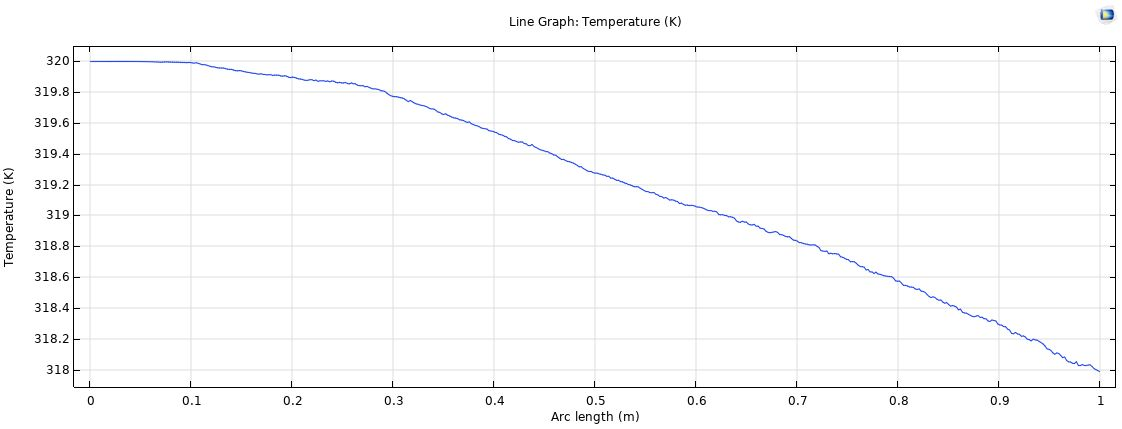
\includegraphics[width=0.47\linewidth]{figures/m2d_4_prof.png}\\
\multicolumn{2}{c}{\small Mesh 4: free quadrilateral, extra fine}\\[3pt]
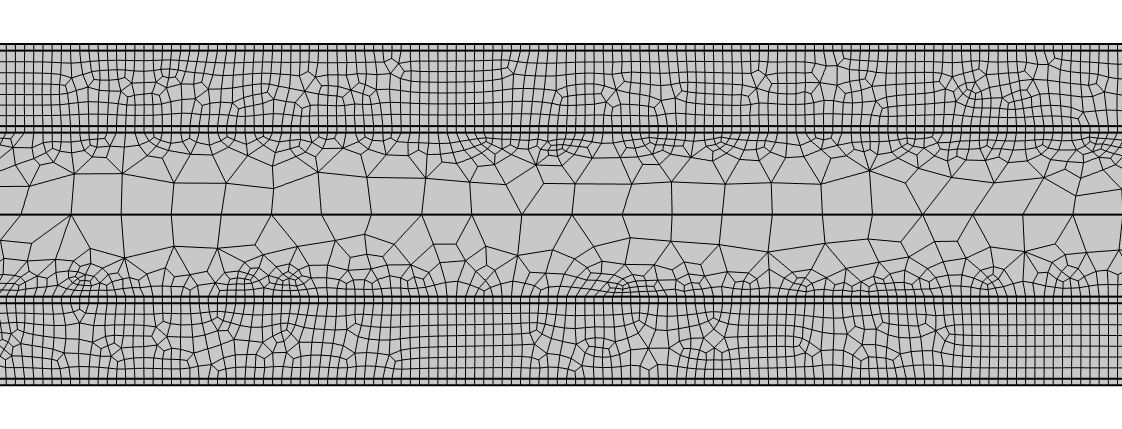
\includegraphics[width=0.47\linewidth]{figures/m2d_5_mesh.jpg} & 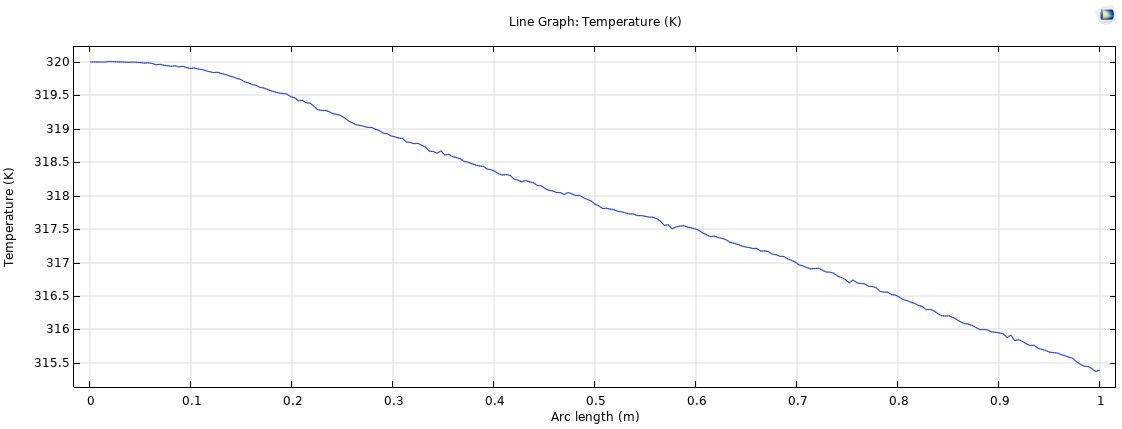
\includegraphics[width=0.47\linewidth]{figures/m2d_5_prof.png}\\
\multicolumn{2}{c}{\small Mesh 5: free quadrilateral, graded}
\end{tabular}
\caption{2D Meshes 4 and 5.}
\end{figure}
\end{document}
